\documentclass[11pt]{scrartcl}
\usepackage[utf8]{inputenc}
\usepackage[ngerman]{babel}
\usepackage{amsmath}
\usepackage{amssymb}
\usepackage{mathtools}
\usepackage{enumitem}
\usepackage{tabularray}

\makeatletter
\newcommand{\qed}{\@ifstar\@qedwhite\@qedblack}
\DeclareRobustCommand{\@qedblack}{%
        \ifmmode \tag*{$\blacksquare$}%
        \else \leavevmode\unskip\penalty9999 \hbox{}\nobreak\hfill\quad\hbox{$\blacksquare$}%
        \fi%
}
\DeclareRobustCommand{\qedwhite}{%
        \ifmmode \tag*{$\Box$}%
        \else \leavevmode\unskip\penalty9999 \hbox{}\nobreak\hfill\quad\hbox{$\Box$}%
        \fi%
}
\makeatother

\newcommand{\N}{\mathbb{N}}
\newcommand{\Q}{\mathbb{Q}}
\newcommand{\R}{\mathbb{R}}
\newcommand{\C}{\mathbb{C}}

%====================================================================
% SETZEN SIE HIER DIE NUMMER DES ÜBUNGSBLATTES UND IHRE(N) NAMEN EIN
% FILL IN THE SHEET NUMBER AND YOUR NAME(S)
%====================================================================
\newcommand{\sheetNum}{3} % Nummer des Übungsblatt / Sheet number
\newcommand{\studentOne}{Alexandros Paraskevaidis} % Name 1
\newcommand{\studentTwo}{Elias Gestrich} % Name 2
%====================================================================

\setkomafont{sectioning}{\normalfont\normalcolor\bfseries}
\usepackage[left=2.5cm,right=2.5cm,top=2.0cm,bottom=2.5cm]{geometry}

% Hyperlinks
\usepackage{hyperref}

% Pseudocode
\usepackage[german,vlined,longend,ruled,linesnumbered]{algorithm2e}
\SetKw{KwDownTo}{downto}
\SetKw{KwAnd}{and}
\SetKw{KwOr}{or}
\DontPrintSemicolon

% Grafiken
\usepackage{graphicx}
\graphicspath{{img/}}
\usepackage{tikz}

% Makros für Aufgaben und Teilaufgaben
\usepackage{marginnote}
\reversemarginpar
\setlength{\parindent}{0cm}
\newcommand{\task}[1]{\subsubsection*{#1}}
\newcommand{\subtask}[1]{\marginnote{#1)}}


\begin{document}

%====================================================================
\begin{small}
\begin{minipage}{0.5 \linewidth}
  Algorithmen und Datenstrukturen\\
  Sommersemester 2024
\end{minipage}
\begin{minipage}{0.5\linewidth}
  \begin{flushright}
    \studentOne\\
    \studentTwo
  \end{flushright}
\end{minipage}
\end{small}
\begin{center}
\begin{sffamily}\Large\bfseries \sheetNum. Übungsblatt\end{sffamily}
\end{center}
%====================================================================

\task{Aufgabe 1 - Pipelines}
Man kann mittels QuickSelect den Median in O(n) finden und dort seine Pipeline verlegen. Dafür erstellen wir ein Array mit der gleichen Größe wie die Anzahl der y-Koordinaten. Wir suchen uns ein zufälliges Pivot Element aus und ordnen alles kleinere links davon und alles größere rechts davon. Falls unser Pivot Element in der Mitte des Arrays landet sind wir fertig. Sonst führen wenden wir unseren bisherigen Algorithmus auf die linke oder rechte Hälfte je nachdem, ob unser Pivot Element kleiner oder größer ist als das Element in der Mitte. Wir machen solange weiter bis unser Pivot Element in der Mitte des Subarrays ist. (Bei Arrays mit gerader Anzahl von Elementen nehmen wir das Element bei $\lfloor(n + 1)/2\rfloor$) \\
Die Pipeline legen wir auf der y-Koordinate. Alle y-Anlegekoordinaten oberhalb würden die Länge der unteren Hälfte der Zuleitungen verlängern und alles unterhalb die Länge der oberen Hälfte verlängern.

\task{Aufgabe 2 - Vorsortiert}

$ A,B $ sortiert mit jeweils $ n $ Elementen $\rightarrow A\left[ \left\lfloor \frac{ n }{ 2 }  \right\rfloor \right] $ Media von $ A $, $ B\left[\left\lfloor \frac{n}{2} \right\rfloor\right] $ Median von $ B $ $\rightarrow$ Media liegt zwischen $ A \left[ \left\lfloor \frac{ n }{ 2 }  \right\rfloor \right] $ und $ B\left[ \left\lfloor \frac{ n }{ 2 }  \right\rfloor\right] $, da sonst mehr als $\frac{n}{2} + \frac{n}{2}$ größer/kleiner - Widerspruch \\
Wenn $ A \left[ \left\lfloor \frac{ n }{ 2 }  \right\rfloor  \right] = B \left[ \left\lfloor \frac{ n }{ 2 }  \right\rfloor  \right] $, dann haben wir unseren Median schon gefunden.
Sonst \OE $A\left[\left\lfloor\frac{n}{2}\right\rfloor\right] < B\left[\left\lfloor\frac{n}{2}\right\rfloor\right] $, der Median liegt also in $ A\left[\left\lfloor\frac{n}{2}\right\rfloor, \dotsc, n \right] $ oder $ B \left[1, \dotsc, \left\lfloor \frac{ n }{ 2 }  \right\rfloor  \right] $ \\
Wenn wir $ A \left[ \left\lfloor \frac{3n}{ 4 }  \right\rfloor  \right] $ und $ B \left[ \left\lfloor \frac{ n }{ 2 }  \right\rfloor  \right] $ vergleichen und sie gleich sind dann haben wir den Media gefunden, da $\frac{3n}{4} + \frac{n}{4}$ kleiner/größer. \\
Wenn $ A \left[ \left\lfloor \frac{3n}{ 4 }  \right\rfloor  \right] < B \left[ \left\lfloor \frac{ n }{ 4 }  \right\rfloor  \right] $, dann liegt der Median in $ A \left[ \left\lfloor \frac{ 3n }{ 4 }  \right\rfloor, \dotsc, n \right] $ oder $ B \left[ 1, \dotsc, \left\lfloor \frac{ n }{ 4 }  \right\rfloor \right] $,
sonst in $ A \left[ \left\lfloor \frac{ n }{ 2 }  \right\rfloor, \dotsc, \left\lfloor \frac{3n}{ 4 }  \right\rfloor  \right] $,
oder $ B \left[ \left\lfloor \frac{ n }{ 4 }  \right\rfloor, \dotsc, \left\lfloor \frac{ n }{ 2 }  \right\rfloor  \right] $

\task{Aufgabe 3 - Heaps und Suchbäume}

    \subtask{a}
    1) So ein Heap ist nicht möglich, da wir immer erst links einfügen müssten aufgrund der notwendigen Linksvollständigkeit für einen Heap. Diese Elemente müssen aber größer sein als ihr Elternknoten, wodurch die Eigenschaft des Binärensuchbaums verletzt wird. \\

    2) Sobald ein kleineres Kind links von einem Elternknoten eingefügt wird, wird die Heapeigenschaft verletzt. Somit ist ein solcher Baum leicht konstruierbar.
    \begin{figure}[h]
    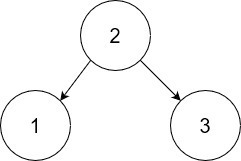
\includegraphics[scale = 0.5]{BaumOhneHeap.jpg}
    \centering
    \end{figure}

    3) So ein BST ist nicht umsetztbar, da ein linksvollständiger BST zwangsweise Kinderknoten enthält, die größer sind als ihre Elternknoten, womit die Heap Eigenschaft verletzt wird.

    \subtask{b}
    Best Case: am wenigsten Vergleiche: Für das $ (k + 1) $-te Element, sind schon $ k $ Elemente im Binärem Suchbaum.
    D.h. im Best Case $ \left\lfloor \log _2(k) \right\rfloor $, also $ \left\lfloor \log _2(k) \right\rfloor  $ Vergleiche.
    Also $ \Omega( n \log (n) ) $.\\
    Würde es nicht balanciert, dann müsste für ein Element, das es unbalanciert macht, mindestens $ \left\lfloor \log _2(n) \right\rfloor + 1 $ Vergleiche gemacht werden.
    Also ist der Best Case $ \Omega(n \log(n)) $

    \newpage
    \task{Aufgabe 4 - Pfade im Suchbaum}

    \subtask{a}
    1) Ein solcher BST existiert, da jeder linke Teilbaum nur Elemente enthält, die kleiner sind als der Elternknoten und jeder rechter Teilbaum nur Elemente enthält, die größer als ihr Elternknoten sind.
    2) Ein solcher BST kann aus demselben Grund existiert wie in 1)
    3) Ein solcher BST ist nicht valide, da bei der Einfügung von Schlüssel 666, der im linken Teilbaum vom Schlüssel 652 auftaucht und somit größer als der Knoten 652 ist, die BST Eigenschaft verletzt.
    4) Ein solcher BST existiert, da keine Eigenschaften des BST verletzt werden.

    \subtask{b}
    Man fängt vom Ende des Arrays an und läuft nach links und merkt sich Minimum und Maximum. Beim Finden eines größeren/kleineren Wertes aktualisiert man entsprechend den aktuellen Max./Min. Wert. Wenn ein Wert auftaucht, der zwischen Maximum und Minimum liegt kann es einen solchen Baum nicht geben, da entsprechend, die Eigenschaft des BST verletzt wird, dass im linken Teilbaum nur größere Elemente vorkommen oder dass im rechten Teilbaum nur kleinere Elemente stehen können.

    \begin{algorithm}[H]
    \caption{BSTCheck (int[] $A$)}
    $max \leftarrow A[k]$\;
    $min \leftarrow A[k]$\;
    \For{$i=k-1$ \KwTo $A[0]$}{
    \uIf{A[i] \textless A[i-1]}{
    $min \leftarrow A[i]$\;
    }
    \uElseIf{A[i] \textgreater A[i-1]}{
    $max \leftarrow A[i]$\;
    }
    \uElse{
    \Return false\;
    }
}
\end{algorithm}

\end{document}
